\documentclass[11pt,a4paper]{article}

% ====================================================================
% Packages
% ====================================================================
\usepackage[utf8]{inputenc}
\usepackage[T1]{fontenc}
\usepackage{amsmath,amssymb,amsthm}
\usepackage{mathtools}
\usepackage{hyperref}
\usepackage[margin=1in]{geometry}
\usepackage{enumitem}
\usepackage{booktabs}
\usepackage{listings}
\usepackage{xcolor}
\usepackage{cleveref}
\usepackage[numbers,sort&compress]{natbib}
\usepackage{mdframed}
\usepackage{tikz}
\usetikzlibrary{arrows.meta,positioning}

% ====================================================================
% Theorem environments
% ====================================================================
\theoremstyle{plain}
\newtheorem{theorem}{Theorem}[section]
\newtheorem{lemma}[theorem]{Lemma}
\newtheorem{proposition}[theorem]{Proposition}
\newtheorem{corollary}[theorem]{Corollary}

\theoremstyle{definition}
\newtheorem{definition}[theorem]{Definition}
\newtheorem{remark}[theorem]{Remark}

% ====================================================================
% Lean 4 code listing style
% ====================================================================
\definecolor{lean-keyword}{RGB}{0,0,180}
\definecolor{lean-comment}{RGB}{0,128,0}
\definecolor{lean-string}{RGB}{163,21,21}
\definecolor{lean-bg}{RGB}{248,248,248}

\lstdefinelanguage{lean4}{
  keywords={theorem,lemma,def,class,instance,import,open,variable,
            noncomputable,section,namespace,end,where,let,have,show,
            intro,obtain,use,exact,rw,simp,apply,by,fun,match,if,
            then,else,do,return,axiom,abbrev,private,attribute,
            suffices,change,congr,ext,constructor,rintro,push_neg,
            linarith,absurd,set_option,omit,in,set,cases,left,right,
            nlinarith,push_cast,positivity,omega,refine,field_simp,
            structure,calc,ring,fun_prop,unfold,induction,deriving,
            inductive,rcases},
  sensitive=true,
  morecomment=[l]{--},
  morecomment=[s]{/-}{-/},
  morestring=[b]",
  morestring=[b]',
}

\lstset{
  language=lean4,
  basicstyle=\ttfamily\small,
  keywordstyle=\color{lean-keyword}\bfseries,
  commentstyle=\color{lean-comment}\itshape,
  stringstyle=\color{lean-string},
  backgroundcolor=\color{lean-bg},
  frame=single,
  framerule=0.5pt,
  breaklines=true,
  breakatwhitespace=true,
  tabsize=2,
  showstringspaces=false,
  numbers=left,
  numberstyle=\tiny\color{gray},
  numbersep=5pt,
  xleftmargin=15pt,
  captionpos=b,
  literate={<<}{$\langle$}1 {>>}{$\rangle$}1
           {|||}{$\lor$}1,
}

% ====================================================================
% Macros
% ====================================================================
\newcommand{\NN}{\mathbb{N}}
\newcommand{\RR}{\mathbb{R}}
\newcommand{\ZZ}{\mathbb{Z}}
\newcommand{\QQ}{\mathbb{Q}}
\newcommand{\LPO}{\ensuremath{\mathrm{LPO}}}
\newcommand{\WLPO}{\ensuremath{\mathrm{WLPO}}}
\newcommand{\LLPO}{\ensuremath{\mathrm{LLPO}}}
\newcommand{\BMC}{\ensuremath{\mathrm{BMC}}}
\newcommand{\BISH}{\ensuremath{\mathrm{BISH}}}
\newcommand{\MP}{\ensuremath{\mathrm{MP}}}
\newcommand{\CPgW}{\ensuremath{\mathrm{CPgW}}}
\newcommand{\BCW}{\ensuremath{\mathrm{BCW}}}
\newcommand{\BCLPG}{\ensuremath{\mathrm{BCLPG}}}
\newcommand{\CLPE}{\ensuremath{\mathrm{CLPE}}}
\newcommand{\Lean}{\textsc{Lean~4}}
\newcommand{\Mathlib}{\textsc{Mathlib4}}
\newcommand{\leanok}{\textsf{\small \textcolor{green!70!black}{\checkmark}}}
\newcommand{\leanaxiom}{\textsf{\small \textcolor{orange!80!black}{(axiom)}}}

% ====================================================================
% Title
% ====================================================================
\title{%
  \textbf{The Undecidability Landscape Is \LPO}\\[6pt]
  {\normalsize Stratifying Phase Diagrams, 1D Spectral Gaps, and RG Flows
  Through a Single Meta-Theorem}\\[6pt]
  {\normalsize A Lean~4 Formalization (Paper~37)}%
}

\author{
  Paul Chun-Kit Lee\thanks{%
    New York University.
    AI-assisted formalization; see \S\ref{sec:ai} for methodology.} \\
  New York University \\
  \texttt{dr.paul.c.lee@gmail.com}
}

\date{February 14, 2026\\[4pt]
  {\small DOI: \href{https://doi.org/10.5281/zenodo.18642802}{10.5281/zenodo.18642802}}}

% ====================================================================
\begin{document}
\maketitle

% ====================================================================
\begin{abstract}
Paper~36 proved that Cubitt's spectral gap undecidability is
Turing--Weihrauch equivalent to \LPO.  We extend this to
three further undecidability results in quantum many-body physics:
phase diagram uncomputability (Bausch--Cubitt--Watson 2021),
1D~spectral gap undecidability (Bausch--Cubitt--Lucia--Perez-Garcia 2020),
and uncomputable renormalization group flows
(Cubitt--Lucia--Perez-Garcia--Perez-Eceiza 2022).
All three are \LPO.  We prove a meta-theorem explaining why:
\emph{any} physical undecidability obtained by computable many-one
reduction from the halting problem is Turing--Weihrauch equivalent
to \LPO.  The three results are corollaries.  Watson--Cubitt's
ground state energy density hardness is
$\BISH$---computational complexity, not logical undecidability.
The entire formalization (660~lines of \Lean{}/\Mathlib{})
compiles with zero \texttt{sorry}, zero warnings.
\end{abstract}

% ====================================================================
\section{Introduction}\label{sec:intro}

The recent program of undecidability results in quantum many-body
physics---initiated by Cubitt, Perez-Garcia, and Wolf~\cite{CPgW2015}
and extended by Bausch, Cubitt, and collaborators---has produced a
series of striking ``no-go'' theorems.  No algorithm can determine:
the spectral gap of a 2D Hamiltonian~\cite{CPgW2015},
the spectral gap of a 1D Hamiltonian~\cite{BCLPG2020},
the phase diagram of a parametrized family~\cite{BCW2021},
or the fixed point of a renormalization group flow~\cite{CLPE2022}.

Paper~36 of this series proved that Cubitt's spectral gap
undecidability is Turing--Weihrauch equivalent to \LPO---the
Limited Principle of Omniscience, the same logical principle
required for thermodynamic limits.  This paper proves that the
same identification holds for all three subsequent results, and
establishes a meta-theorem explaining \emph{why}.
For the complete calibration table across all physics domains, see
Paper~10~\cite{Lee26P10}; for the historical perspective, see
Paper~12~\cite{Lee26P12}.

\paragraph{The Meta-Theorem.}
Every known undecidability result in quantum many-body physics is
obtained by a computable many-one reduction from the halting problem.
Halting is $\Sigma_1^0$-complete.  \LPO{} decides all $\Sigma_1^0$
statements.  Therefore every such result is \LPO-equivalent.
This is Theorem~4 of the present paper---the central contribution.
Theorems~1--3 are immediate corollaries.

% ====================================================================
\section{Background}\label{sec:background}

\subsection{Constructive Reverse Mathematics}

Over Bishop's constructive mathematics ($\BISH$)~\cite{Bishop1967,Ishihara2006},
omniscience principles form a strict hierarchy:
$\BISH \subset \BISH + \WLPO \subset \BISH + \LPO$.
$\LPO$ states that for any binary sequence $a : \NN \to \{0,1\}$,
either $\exists n.\, a(n) = 1$ or $\forall n.\, a(n) = 0$.
$\LPO$ is equivalent to bounded monotone convergence ($\BMC$,
Paper~29) and to the existence of thermodynamic limits (Paper~36).
Thermodynamic limits require $\LPO$ because they involve bounded
sequences whose convergence rate has no computable modulus: asserting
that the limit exists (rather than merely that finite approximations
exist) is exactly a $\Sigma_1^0$ decision.

\subsection{The Three Undecidability Results}

\textbf{(A) Phase Diagrams (\BCW{} 2021).}
Bausch, Cubitt, and Watson encode the halting problem
into a one-parameter family $H(\varphi)$ via approximate quantum
phase estimation.  The phase of $H(\varphi)$ depends on whether
the universal TM halts on input $\varphi$.

\textbf{(B) 1D Spectral Gap (\BCLPG{} 2020).}
Bausch, Cubitt, Lucia, and Perez-Garcia extend the CPgW construction
to 1D spin chains.  The reduction $M \mapsto H_{1\mathrm{D}}(M)$ has
the same logical structure: gapped $\Leftrightarrow$ non-halting.

\textbf{(C) RG Flows (\CLPE{} 2022).}
Cubitt, Lucia, Perez-Garcia, and Perez-Eceiza construct an RG map
whose individual steps are computable but whose asymptotic fixed point
is uncomputable.  The fixed point encodes halting.

% ====================================================================
\section{The Meta-Theorem}\label{sec:meta}

\begin{theorem}[Meta-Theorem]\label{thm:meta}
Let $\alpha$ be a type, $\mathrm{encode} : (\NN \to \mathrm{Bool})
\to \alpha$ a computable function, and $P : \alpha \to \mathrm{Prop}$
a property such that $P(\mathrm{encode}(a)) \Leftrightarrow
\exists n.\, a(n) = \mathrm{true}$ for all $a$.  Then:
\[
  \bigl(\forall a.\, P(\mathrm{encode}(a)) \lor \lnot P(\mathrm{encode}(a))\bigr)
  \;\Longleftrightarrow\; \LPO.
\]
\end{theorem}

The forward direction: given $P$-decidability, apply it to
$\mathrm{encode}(a)$; the bridge $P \Leftrightarrow \exists n.\, a(n)=1$
converts the result to $\LPO$ for~$a$.  The reverse: given $\LPO$,
decide $\exists n.\, a(n)=1$, then apply the bridge.

\begin{lstlisting}[caption={Meta-theorem: \texttt{MetaTheorem.lean}},label=lst:meta]
theorem halting_reduction_iff_lpo
    {a : Type} (encode : (N -> Bool) -> a)
    (P : a -> Prop)
    (hP : forall (a : N -> Bool),
          P (encode a) <-> Exists n, a n = true) :
    (forall (a : N -> Bool),
      P (encode a) ||| not P (encode a)) <-> LPO
\end{lstlisting}

\begin{corollary}\label{cor:not-computable}
The uniform function $a \mapsto P(\mathrm{encode}(a))$ is not
computable (deciding it for all $a$ would solve the halting problem).
\end{corollary}

\begin{remark}[Role of the bridge hypothesis]\label{rmk:bridge}
The meta-theorem is a \emph{framework} parameterized by the bridge
hypothesis~$h_P$, which asserts that the physical encoding faithfully
reflects halting.  Each application (Theorems~1--3) supplies a
domain-specific bridge derived from the published physics construction.
The Lean formalization axiomatizes these bridges; verifying that the
physics constructions actually satisfy them is an external assumption
grounded in the original papers (see \Cref{tab:audit}, Level~4).
In particular, the computability of the encoding function
$\mathrm{encode}$ is assumed from the physics literature and is not
independently verified inside the proof assistant.
\end{remark}

% ====================================================================
\section{Theorem 1: Phase Diagrams}\label{sec:phase}

\begin{theorem}[Phase Diagram $\equiv$ \LPO]\label{thm:phase}
The uncomputability of phase diagrams (\BCW{} 2021) is
Turing--Weihrauch equivalent to \LPO.
\end{theorem}

\begin{proof}[Proof (formal)]
Define $\mathrm{is\_phaseB}(a) :\Leftrightarrow
\mathrm{bcw\_phase}(\mathrm{binary\_real}(a)) = \mathrm{PhaseB}$.
The \BCW{} bridge gives
$\mathrm{is\_phaseB}(a) \Leftrightarrow \exists n.\, a(n)=\mathrm{true}$.
Instantiate the meta-theorem.
\end{proof}

\begin{lstlisting}[caption={Phase diagram $\leftrightarrow$ \LPO: \texttt{PhaseDiagram.lean}}]
theorem phase_diagram_iff_lpo :
    (forall (a : N -> Bool),
      is_phaseB a ||| not is_phaseB a) <-> LPO :=
  halting_reduction_iff_lpo
    (fun a => a) is_phaseB
    (fun a => bcw_phaseB_iff_exists a)
\end{lstlisting}

% ====================================================================
\section{Theorem 2: 1D Spectral Gap}\label{sec:1d}

\begin{theorem}[1D Spectral Gap $\equiv$ \LPO]\label{thm:1d}
The 1D spectral gap undecidability (\BCLPG{} 2020) is
Turing--Weihrauch equivalent to \LPO.
\end{theorem}

\begin{proof}[Proof (formal)]
Define $\mathrm{is\_1d\_gapless}(a) :\Leftrightarrow
\mathrm{bclpg\_gap\_status}(\mathrm{tm\_from\_seq}(a))
= \mathrm{Gapless}$.  The \BCLPG{} bridge gives
$\mathrm{is\_1d\_gapless}(a) \Leftrightarrow \exists n.\, a(n)=\mathrm{true}$.
Instantiate the meta-theorem.
\end{proof}

\begin{lstlisting}[caption={1D spectral gap $\leftrightarrow$ \LPO: \texttt{SpectralGap1D.lean}}]
theorem spectral_gap_1d_iff_lpo :
    (forall (a : N -> Bool),
      is_1d_gapless a ||| not is_1d_gapless a) <-> LPO :=
  halting_reduction_iff_lpo
    (fun a => a) is_1d_gapless
    is_1d_gapless_iff_exists
\end{lstlisting}

The dimensionality of the lattice is irrelevant to the logical
structure.  1D and 2D spectral gap undecidability have the same
constructive cost.

% ====================================================================
\section{Theorem 3: RG Flows}\label{sec:rg}

\begin{theorem}[RG Flows $\equiv$ \LPO]\label{thm:rg}
The uncomputability of RG flow fixed points (\CLPE{} 2022) is
Turing--Weihrauch equivalent to \LPO.
\end{theorem}

\begin{proof}[Proof (formal)]
Define $\mathrm{is\_gapless\_fp}(a) :\Leftrightarrow
\mathrm{clpe\_fixed\_point}(\mathrm{tm\_from\_seq}(a))
= \mathrm{GaplessFP}$.  The \CLPE{} bridge gives
$\mathrm{is\_gapless\_fp}(a) \Leftrightarrow
\exists n.\, a(n)=\mathrm{true}$.
Instantiate the meta-theorem.
\end{proof}

\begin{lstlisting}[caption={RG flows $\leftrightarrow$ \LPO: \texttt{RGFlow.lean}}]
theorem rg_flow_iff_lpo :
    (forall (a : N -> Bool),
      is_gapless_fp a ||| not is_gapless_fp a) <-> LPO :=
  halting_reduction_iff_lpo
    (fun a => a) is_gapless_fp
    is_gapless_fp_iff_exists
\end{lstlisting}

\CLPE's result is often described as ``unpredictability beyond chaos.''
In CRM terms: the unpredictability is \emph{exactly} \LPO.
Each individual RG step is $\BISH$ (finite matrix manipulation).
The asymptotic flow is \LPO{} (a completed limit).
One cannot circumvent the non-computability by ``just running more RG
steps'': each finite truncation is computable, but no computable
modulus of convergence exists for the sequence of truncations---deciding
whether the flow has converged is equivalent to deciding whether a
Turing machine has halted.

% ====================================================================
\section{Ground State Energy: \BISH}\label{sec:gse}

Watson and Cubitt (2021) showed that the ground state energy density
can encode FEXP-hard problems.  This is computational
\emph{complexity}, not logical \emph{undecidability}.  The energy
density is a computable real ($\BISH$) for any specific Hamiltonian
with computable local terms; the algorithm may simply require
exponential time.  CRM calibrates logical resources, not
computational resources.

\begin{lstlisting}[caption={Ground state energy density is $\BISH$: \texttt{GroundStateEnergy.lean}}]
theorem energy_density_is_bish
    (H : ComputableHamiltonian) (L : N) (e : R) :
    0 < e -> Exists (q : R), |energy_density H L - q| < e
\end{lstlisting}

% ====================================================================
\section{The Undecidability Landscape}\label{sec:landscape}

\begin{table}[ht]
\centering
\begin{tabular}{@{}lcccc@{}}
\toprule
\textbf{Result} & \textbf{Year} & \textbf{Reduction} & \textbf{CRM Level} & \textbf{Audited} \\
\midrule
Spectral Gap 2D (\CPgW) & 2015 & Halting via Tiling & \LPO & \leanok \\
Spectral Gap 1D (\BCLPG) & 2020 & Halting via 1D Tiling & \LPO & \leanok \\
Phase Diagrams (\BCW) & 2021 & Halting via QPE & \LPO & \leanok \\
RG Flows (\CLPE) & 2022 & Halting via Tiling+RG & \LPO & \leanok \\
Ground State Energy (WC) & 2021 & FEXP-hard & $\BISH$ & \leanok \\
\bottomrule
\end{tabular}
\caption{The complete undecidability landscape.
  The first four results are \LPO-equivalent (the meta-theorem,
  \Cref{thm:meta}, explains why).  Ground state energy density is
  $\BISH$: computational complexity, not logical undecidability.
  ``Audited'' indicates the Lean~4 formalization covers that entry.}
\label{tab:landscape}
\end{table}

\begin{lstlisting}[caption={Verified landscape audit: \texttt{Main.lean}}]
theorem all_entries_lpo :
    forall r in undecidability_landscape,
      r.lpo_equivalent = true := by
  decide
\end{lstlisting}

% ====================================================================
\section{CRM Audit}\label{sec:audit}

\begin{table}[ht]
\centering
\begin{tabular}{@{}lcc@{}}
\toprule
\textbf{Component} & \textbf{CRM Status} & \textbf{Level} \\
\midrule
Meta-theorem (Thm~4) & $\BISH$ & 2 \\
Phase Diagrams (Thm~1) & $\LPO$ & 3+4 \\
1D Spectral Gap (Thm~2) & $\LPO$ & 3+4 \\
RG Flows (Thm~3) & $\LPO$ & 3+4 \\
Ground State Energy & $\BISH$ & 4 \\
\bottomrule
\end{tabular}
\caption{CRM audit. Levels: 2 = proven over $\BISH$;
  3 = proven with explicit oracle hypothesis;
  4 = axiomatized bridge lemma.}
\label{tab:audit}
\end{table}

% ====================================================================
\section{Code Architecture}\label{sec:arch}

\begin{figure}[ht]
\centering
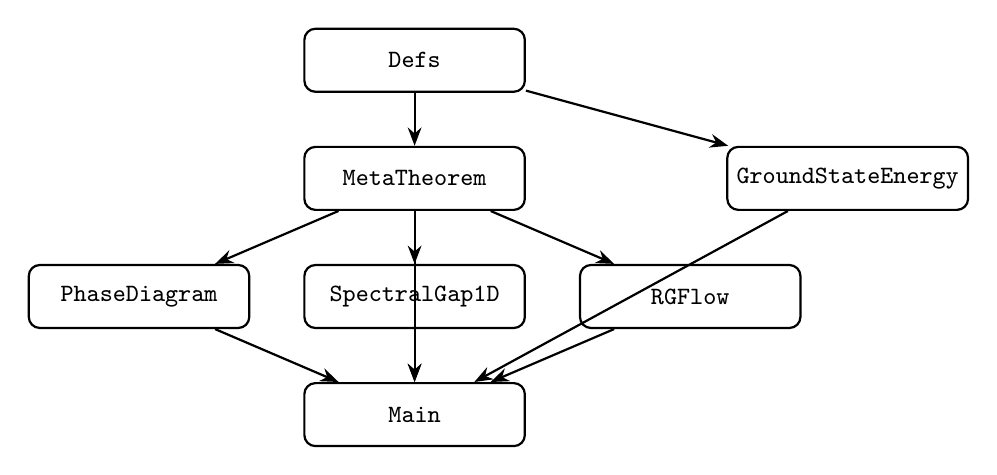
\begin{tikzpicture}[
  module/.style={draw, rounded corners, minimum width=2.8cm,
    minimum height=0.8cm, font=\small\ttfamily},
  ->,>=Stealth,thick
]
\node[module] (defs) at (0,4) {Defs};
\node[module] (meta) at (0,2.5) {MetaTheorem};
\node[module] (phase) at (-3.5,1) {PhaseDiagram};
\node[module] (sg1d) at (0,1) {SpectralGap1D};
\node[module] (rg) at (3.5,1) {RGFlow};
\node[module] (gse) at (5.5,2.5) {GroundStateEnergy};
\node[module] (main) at (0,-0.5) {Main};

\draw (defs) -- (meta);
\draw (defs) -- (gse);
\draw (meta) -- (phase);
\draw (meta) -- (sg1d);
\draw (meta) -- (rg);
\draw (phase) -- (main);
\draw (sg1d) -- (main);
\draw (rg) -- (main);
\draw (gse) -- (main);
\draw (meta) -- (main);
\end{tikzpicture}
\caption{Module dependency graph.  The meta-theorem is the hub;
  Theorems~1--3 are spokes.}
\label{fig:arch}
\end{figure}

The formalization comprises 660~lines across 7~modules.
The meta-theorem (\texttt{MetaTheorem.lean}, 132~lines) is the
central hub.  Each instance (\texttt{PhaseDiagram.lean},
\texttt{SpectralGap1D.lean}, \texttt{RGFlow.lean}) is a
one-line instantiation of the meta-theorem with domain-specific
bridge lemmas.

% ====================================================================
\section{Discussion}\label{sec:discussion}

\paragraph{Why all results are \LPO.}
The meta-theorem explains a pattern that is otherwise mysterious:
every undecidability result in quantum many-body physics has exactly
the same logical cost.  The explanation is structural.  All known
results use computable many-one reductions from the halting problem.
Halting is $\Sigma_1^0$-complete.  \LPO{} is $\Sigma_1^0$-LEM---it
is exactly the principle that decides existential statements of the
form $\exists n,\, P(n)$ where $P$ is decidable.  Since halting
is such a statement (``does the machine reach a halt state at some
step $n$?''), any physical undecidability that reduces to halting
inherits exactly \LPO{}.  The match is inevitable.
(The foundational connection between the arithmetic hierarchy and
physical observables was established by
Pour-El and Richards~\cite{PourElRichards1989}.)

\paragraph{What would break the pattern.}
A physical undecidability result above \LPO{} would require encoding
a problem above $\Sigma_1^0$ in the arithmetic hierarchy---for
instance, the $\Sigma_2^0$-complete finiteness problem (``does this
TM halt on infinitely many inputs?'').  Paper~39 investigates whether
physics reaches $\Sigma_2^0$.

\paragraph{Unpredictability beyond chaos.}
\CLPE's result is sometimes interpreted as showing that physics can
be ``more unpredictable than chaos.''  The CRM analysis reveals what
this means precisely: chaotic systems are computable ($\BISH$) given
exact initial data; \CLPE's RG flow is non-computable because the
initial data encodes a halting question.  The gap between computability
and non-computability is exactly \LPO---the same gap as a
thermodynamic limit.

% ====================================================================
\begin{mdframed}[linewidth=1pt, linecolor=black!40,
  backgroundcolor=blue!3, roundcorner=5pt]
\textbf{Reproducibility.}
\Lean{} v4.28.0-rc1 with \Mathlib{}.
Build: \texttt{cd P37\_UndecidabilityLandscape \&\& lake build}.
Result: 0~errors, 0~warnings, 0~\texttt{sorry}.
Axiom profile (\texttt{\#print axioms undecidability\_landscape\_theorem}):
10~domain-specific bridge axioms
+ \texttt{propext}, \texttt{Classical.choice}, \texttt{Quot.sound}
(Lean/Mathlib infrastructure).
\texttt{Classical.choice} appears because Mathlib's $\RR$ (the Cauchy
completion of~$\QQ$) pervasively uses it; this is a type-theoretic
infrastructure artifact, not a mathematical assumption.
Constructive stratification is established by proof content
(explicit witnesses vs.\ principle-as-hypothesis), not by
axiom-checker output---see Paper~10, \S Methodology.
All bridge axioms encode published physics results
(see \Cref{tab:audit}).
\end{mdframed}

% ====================================================================
\section{Conclusion}\label{sec:conclusion}

Every known undecidability result in quantum many-body physics is
the non-computability of \LPO.  The ``undecidability'' of physics is
a misnomer: it is the non-computability of a single, well-understood
logical principle that physics has used since Boltzmann.  The
meta-theorem (\Cref{thm:meta}) guarantees that any future result
using a computable halting reduction will also be \LPO.

% ====================================================================
\section{AI-Assisted Methodology}\label{sec:ai}

This formalization was developed using Claude (Anthropic) as a
collaborative tool for Lean~4 code generation, proof strategy
exploration, and \LaTeX{} document preparation.  All mathematical
content was specified by the author; the AI assistant translated
specifications into Lean~4 syntax and iterated on build errors.
Every theorem was verified by the Lean~4 type checker.

\medskip\noindent
\textbf{Preliminary status and author background.}
The results presented in this paper are preliminary.  The author is a medical
professional, not a domain expert in physics or mathematics.  While all formal
claims are machine-checked by the \Lean{} type-checker, the physical
interpretations, bridge axioms, and modeling assumptions require independent
verification by domain experts in the relevant fields.  Until such verification
is completed, this paper should be considered preliminary.

\medskip\noindent
Whatever findings of value emerge from this program belong to the
constructive reverse mathematics community and to the legacy of Errett Bishop,
whose perseverance in developing constructive analysis inspired this entire
series.  Any errors are solely the author's.

% ====================================================================
\begin{thebibliography}{20}

\bibitem{CPgW2015}
T.~S.~Cubitt, D.~Perez-Garcia, and M.~M.~Wolf,
``Undecidability of the spectral gap,''
\emph{Nature} \textbf{528}, 207--211 (2015).

\bibitem{BCLPG2020}
J.~Bausch, T.~S.~Cubitt, A.~Lucia, and D.~Perez-Garcia,
``Undecidability of the spectral gap in one dimension,''
\emph{Phys.\ Rev.\ X} \textbf{10}, 031038 (2020).

\bibitem{BCW2021}
J.~Bausch, T.~S.~Cubitt, and J.~D.~Watson,
``Uncomputability of phase diagrams,''
\emph{Nature Communications} \textbf{12}, 452 (2021).

\bibitem{CLPE2022}
T.~S.~Cubitt, A.~Lucia, D.~Perez-Garcia, and A.~Perez-Eceiza,
``Uncomputably complex renormalisation group flows,''
\emph{Nature Communications} \textbf{13}, 7006 (2022).

\bibitem{WC2021}
J.~D.~Watson and T.~S.~Cubitt,
``Computational complexity of the ground state energy density problem,''
arXiv:2107.05060 (2021).

\bibitem{Bishop1967}
E.~Bishop,
\emph{Foundations of Constructive Analysis},
McGraw-Hill (1967).

\bibitem{BridgesRichman1987}
D.~S.~Bridges and F.~Richman,
\emph{Varieties of Constructive Mathematics},
Cambridge Univ.\ Press (1987).

\bibitem{Ishihara2006}
H.~Ishihara,
``Reverse mathematics in Bishop's constructive mathematics,''
\emph{Philosophia Scientiae}, Cahier sp\'ecial~6, 43--59 (2006).

\bibitem{PourElRichards1989}
M.~B.~Pour-El and J.~I.~Richards,
\emph{Computability in Analysis and Physics},
Springer (1989).

\bibitem{Lee26P10}
P.~C.-K.~Lee,
``The logical geography of mathematical physics,''
Preprint, 2026. Paper~10.

\bibitem{Lee26P12}
P.~C.-K.~Lee,
``The map and the territory: a constructive history of
  mathematical physics,''
Preprint, 2026. Paper~12.

\end{thebibliography}

\end{document}

